
\documentclass[12pt]{article}

\usepackage{graphicx}
\graphicspath{ {./images/} }

\usepackage{epsfig}
\usepackage{amsmath,amsthm}
\usepackage{listings}


\newtheorem{lemma}{Lemma}
\newtheorem{theorem}{Theorem}


\usepackage{titlesec}
\titleformat{\section}
{\normalfont\Large\bfseries}{Question~\thesection:}{1em}{}

\newlength{\toppush}
\setlength{\toppush}{2\headheight}
\addtolength{\toppush}{\headsep}


\def\subjnum{Comp 160}
\def\subjname{Algorithms}


\def\doheading#1#2#3{\vfill\eject\vspace*{-\toppush}%
  \vbox{\hbox to\textwidth{{\bf} \subjnum: \subjname \hfil Erli Cai}%
    \hbox to\textwidth{{\bf} Tufts University, Fall 2020 \hfil#3\strut}%
    \hrule}}


\newcommand{\htitle}[1]{\vspace*{1.25ex plus 1ex minus 0ex}%
\begin{center}
{\large\bf #1}
\end{center}} 

\setlength\parindent{0pt}

\begin{document}
\doheading{2}{title}{Homework 00}

\section{}
a.b.\\

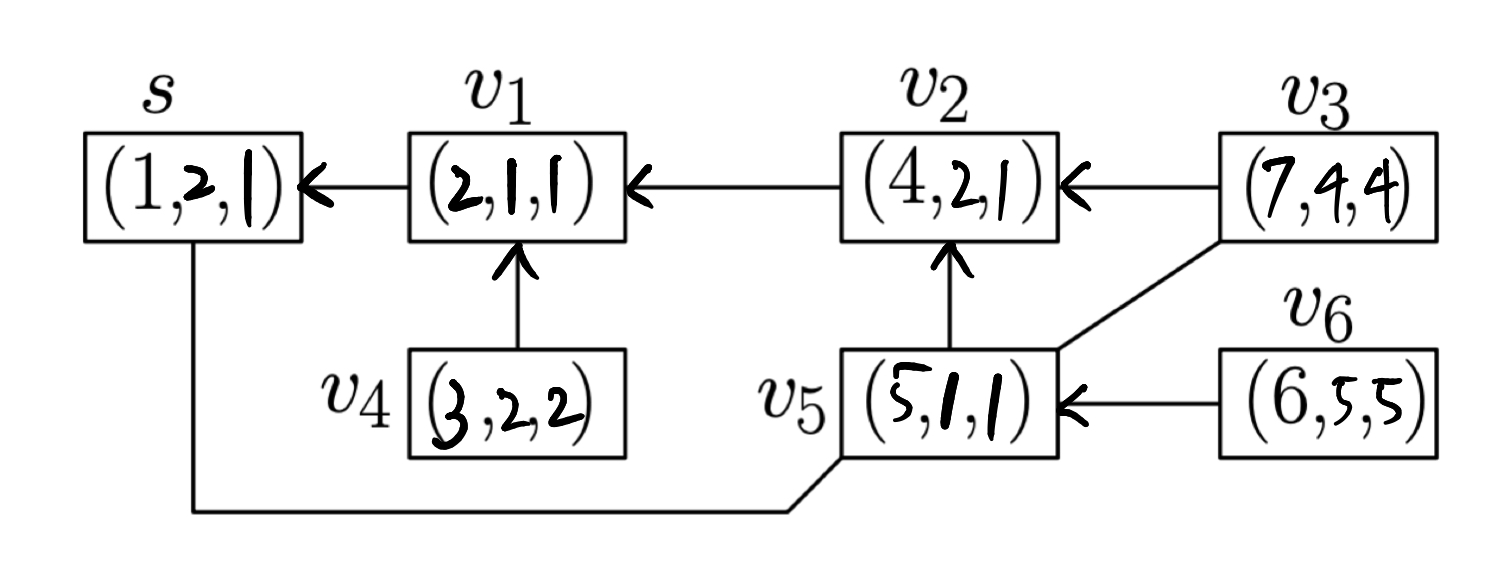
\includegraphics[scale = 0.2]{1.jpg}
\\

c. cut vertices are v1 and v5

v1 is  a cut vertex because $v4.\beta = v1.dics = 2$ and v1 is the parent of v4\\
v5 is  a cut vertex because $v6.\beta = v5.dics = 5$ and v5 is the parent of v6

\pagebreak

\section{}

(a) A simple method would be run Prim's algorithm on $G_2$.\\
Runtime = O((n+1) + (m+n)log(n+1)) = O(n + (m+n)logn)\\
Correctness is guaranteed by the correctness of Prim's algorithm.\\

(b) 
A faster algorithm would be:\\
step1: Find all edges adjacent to v\\
step2: Find the lightest weight edge adjacent to v, call this edge e. \\
Then $T_2 = T_1 + e$ would be a MST for $G_2$\\

Runtime: step 1 will go through all edges of $G_2$, so it will take O(m+n) time. step 2 chooses the lightest weight edge out of O(n) edges, so it takes O(n) time. So this algorithm takes O(m+n) time in total.\\

Correctness:  Firstly, since $G_1$ is a subgraph of $G_2$, we know that the MST for $G_1$ would be a subgraph of MST of $G_2$. By cut lemma, we know that the lightest weight edge adjacent to v will be in MST ( and no other edges adjacent to v). And in lecture we have shown that if $T_1$ is a subset of MST and e is an edge to add, then $T_2 = T_1 + e$ would also be a subset of MST. And since $T_2$ already span edges of $G_2$, it is a MST for $G_2$

\pagebreak

\section{}
We could solve this problem by using Kruskal's algorithm with one small change. Since all the edges' weight are integers in the range 1 to k, we can now use a counting sort to sort the edges. And since this step is the bottle-neck in the Kruskal's algorithm, we could speed up Kruskal's algorithm by doing this.\\

The runtime for counting sort is O(k+n), while in the original Kruskal's algorithm, we need O(mlogm) rumtime\\

So, the runtime is now O(n + (k+n) + nlogn + m) = O(nlogn + m)









\end{document}


